\documentclass[12pt]{article}

\pagestyle{empty}
\setlength{\topmargin}{0in}
\setlength{\headheight}{0in}
\setlength{\topsep}{0in}
\setlength{\textheight}{9in}
\setlength{\oddsidemargin}{0in}
\setlength{\evensidemargin}{0in}
\setlength{\textwidth}{6.5in}

\usepackage{palatino,graphics,amsmath,amssymb,enumitem}

\newcommand{\ds}{\displaystyle}
\newcommand{\vs}[1]{\vspace{#1in}}
\renewcommand{\vss}[1]{\vspace*{#1in}}
\newcommand{\bvec}{{\mathbf b}}
\newcommand{\cvec}{{\mathbf c}}
\newcommand{\dvec}{{\mathbf d}}
\newcommand{\evec}{{\mathbf e}}
\newcommand{\fvec}{{\mathbf f}}
\newcommand{\qvec}{{\mathbf q}}
\newcommand{\uvec}{{\mathbf u}}
\newcommand{\vvec}{{\mathbf v}}
\newcommand{\wvec}{{\mathbf w}}
\newcommand{\xvec}{{\mathbf x}}
\newcommand{\yvec}{{\mathbf y}}
\newcommand{\zvec}{{\mathbf y}}
\newcommand{\zerovec}{{\mathbf 0}}
\newcommand{\real}{{\mathbb R}}
\newcommand{\twovec}[2]{\left[\begin{array}{r}#1 \\ #2
    \end{array}\right]}
\newcommand{\ctwovec}[2]{\left[\begin{array}{c}#1 \\ #2
   \end{array}\right]}
\newcommand{\threevec}[3]{\left[\begin{array}{r}#1 \\ #2 \\ #3
  \end{array}\right]}
\newcommand{\cthreevec}[3]{\left[\begin{array}{c}#1 \\ #2 \\ #3
    \end{array}\right]}
\newcommand{\fourvec}[4]{\left[\begin{array}{r}#1 \\ #2 \\ #3 \\ #4
    \end{array}\right]}
\newcommand{\cfourvec}[4]{\left[\begin{array}{c}#1 \\ #2 \\ #3 \\ #4
    \end{array}\right]}
\newcommand{\mattwo}[4]{\left[\begin{array}{rr}#1 \amp #2 \\ #3 \amp #4 \\ \end{array}\right]}
\renewcommand{\span}[1]{\text{Span}\{#1\}}
\newcommand{\bcal}{{\cal B}}
\newcommand{\ccal}{{\cal C}}
\newcommand{\scal}{{\cal S}}
\newcommand{\wcal}{{\cal W}}
\newcommand{\ecal}{{\cal E}}
\newcommand{\coords}[2]{\left\{#1\right\}_{#2}}
\newcommand{\gray}[1]{\color{gray}{#1}}
\newcommand{\lgray}[1]{\color{lightgray}{#1}}
\newcommand{\rank}{\text{rank}}
\newcommand{\col}{\text{Col}}
\newcommand{\nul}{\text{Nul}}

\begin{document}

\noindent
{\bf Mathematics 227} \\ 
{\bf Exam 1 Review}

\bigskip
\begin{enumerate}
\item Describe the solution space to the linear system:
  $$
  \begin{alignedat}{5}
    2x_1 & {}-{} & x_2 & {}{} & & {}+{} & 3x_4 & {}={} & 6 \\
    x_1 & {}{} & & {}+{} & 3x_3 & {}-{} & x_4 & {}={} & 6 \\
    2x_1 & {}{} & & {}+{} & x_3 & {}+{} & 3x_4 & {}={} & 7 \\
  \end{alignedat}
  $$

  \vs{2}
  Describe the solution space to the vector equation
  $$
  \left[
    \begin{array}{cccc}
      2 & -1 & 0 & 3 \\
      1 & 0 & 3 & -1 \\
      2 & 0 & 1 & 3 \\
    \end{array}
  \right]
  \xvec = \threevec667.
  $$

  \vs{1.25}
  Suppose that
  $$
  \vvec_1=\threevec212, \hspace*{24pt}
  \vvec_2=\threevec{-1}00, \hspace*{24pt}
  \vvec_3=\threevec031, \hspace*{24pt}
  \vvec_4=\threevec3{-1}3, \hspace*{24pt}
  \bvec=\threevec667.
  $$
  Can $\bvec$ be written as a linear combination of $\vvec_1$,
  $\vvec_2$, $\vvec_3$, and $\vvec_4$?  If so, find one set of
  weights.

  \vs{1}
  \newpage
  Is $\bvec$ is $\span{\vvec_1,\vvec_2,\vvec_3,\vvec_4}$?

  \vs{1}
  Describe $\span{\vvec_1,\vvec_2,\vvec_3,\vvec_4}$.  Explain your thinking.

  \vs{1}

\item Give a condition on the pivots 
  \begin{enumerate}[label=(\alph*)]
  \item of an augmented matrix such that the associated linear system
    is not consistent. 

    \vs{0.75}
  \item of an augmented matrix such that the associated linear system
    has a unique solution.

    \vs{0.75}
  \item of a matrix $A$ such that $A\xvec=\bvec$ is
    consistent for any vector $\bvec$.

    \vs{0.75}
  \item of a $10\times10$ matrix $A$ such that the homogeneous
    equation has a unique solution.

    \vs{0.75}
  \end{enumerate}


\item What is the smallest number of vectors that span $\real^{1234}$?
  Explain your thinking.

  \vs{1}

  \newpage
\item Determine if the following matrix is in reduced row echelon
  form.  If not, perform a sequence of row operations to put it in
  reduced row echelon form (without using any computational device).
  Then give a description of the solution space of the associated
  linear system.

  $\ds
  \left[
    \begin{array}{cccc|c}
      0 & 0 & 0 & 0 & 0 \\
      -1 & 2 & 0 & 0 & 3 \\
      0 & 1 & 0 & 1 & -2 \\
    \end{array}
  \right]
  $

  \vs{1}
\item Suppose that $\vvec=\twovec2{-1}$ and $\wvec=\twovec11$.  Sketch
  the vectors $\vvec$, $\wvec$, $2\vvec$, and $\vvec+\wvec$.

  \begin{center}
    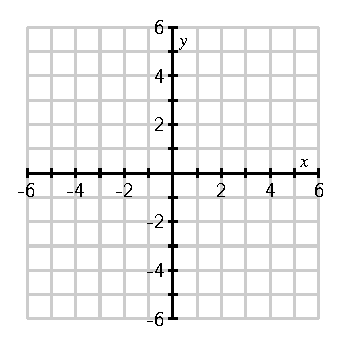
\includegraphics{empty-6.eps}
  \end{center}

  Sketch all vectors of the form $t\vvec$ where $t$ is any scalar.

  \medskip

  Sketch all vectors of the form $\wvec + t\vvec$ where $t$ is any
  scalar.

  \medskip
  \newpage
\item Consider the 2-dimensional vectors $\vvec$ and $\wvec$ shown
  below.

  \begin{center}
    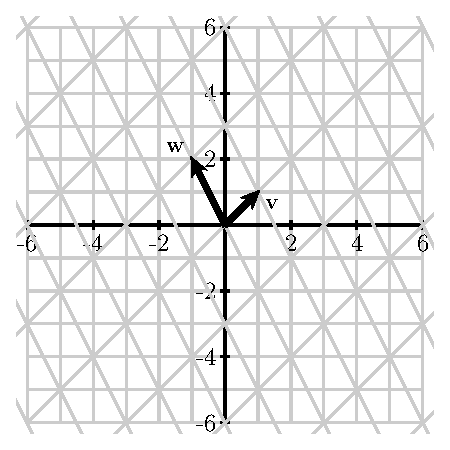
\includegraphics{12-review-fig.eps}
  \end{center}

  Sketch the linear combination $a\vvec + b\wvec$ with weights $a=-3$
  and $b=2$.

  \medskip
  Can the vector $\twovec{3}{-3}$ be written as a linear combination
  of $\vvec$ and $\wvec$?  If so, how?

  \vs{1}
  Describe the solution space to the equation
  $$
  \left[
    \begin{array}{cc}
      \vvec & \wvec \\
    \end{array}
  \right]
  \xvec = \twovec{2}{5}.
  $$

  \vs{1}
  \newpage
\item Determine whether the following statements are true or false 
  including a justification for your response.

  \begin{enumerate}[label=(\alph*)]
  \item If $\vvec_1$, $\vvec_2$, $\vvec_3$ and $\vvec_4$ are vectors
    in $\real^3$, then their span is $\real^3$.

    \vs{1}
  \item Suppose that the span of $\vvec_1,\vvec_2,\ldots,\vvec_{27}$
    is $\real^{27}$.  Then every vector in $\real^{27}$ can be written
    as a linear combination of $\vvec_1,\vvec_2,\ldots,\vvec_{27}$
    is $\real^{27}$ in exactly one way.

    \vs{1.5}
  \item Is $\bvec$ is a linear combination of the vectors $\vvec_1$,
    $\vvec_2$, and $\vvec_3$, then the equation
    $$
    \left[
      \begin{array}{ccc}
        \vvec_1 & \vvec_2 & \vvec_3 \\
      \end{array}
    \right]
    \xvec = \bvec
    $$
    is consistent.
  \end{enumerate}
  

  
    

  

\end{enumerate}


\end{document}
